\documentclass[11p]{article}
\usepackage{amsmath}
\usepackage{amsfonts}
\usepackage{bm}
\usepackage{tikz} 

\tikzset{main/.style = {draw, circle, minimum width={width("$l-1$")+10pt}}}
\tikzset{dashdot/.style = {draw, dashed, circle, minimum width={width("$l-1$")+10pt}}}
%opening
\title{Lignes de bus, approche Markov}
\author{notes GG}

\begin{document}
	
\maketitle
Soit $x_i$, resp. $y_i$, le nombre de passagers qui montent, resp. descendent, en $i$ ($1 \leq i \leq l$). On pose le $n_{i, i+1}$ le nombre de passagers qui sont transportées entre $i$
à $i+1$. On cherche $N_{ij}$ avec les bonnes marges. \\

Posons $p^\text{in}_i$ et $p^\text{out}_i$ comme :

\begin{align}
p^\text{in}_i &:= \frac{x_i}{x_\bullet} \\
p^\text{out}_i &:= \frac{y_i}{n_{i-1, i}} = \frac{y_i}{\sum_{1 \leq k \leq (i-1)} (x_k - y_k)}
\end{align}

On peut alors supposer une distribution $f_{ij} = \frac{N_{ij}}{N_{\bullet \bullet}}$ de la forme suivante :

\begin{equation}
f_{ij} = \begin{cases}
p^\text{in}_i (1 - p^\text{out}_{i+1}) \cdots (1 - p^\text{out}_{j-1}) p^\text{out}_j & \text{si } i < j - 1 \\
p^\text{in}_i p_j^\text{out} & \text{si } i = j - 1 \\
0 & \text{sinon}
\end{cases}
\end{equation}

\section{Chaîne de Markov}

La modélisation par une chaîne de Markov se fait de la façon suivante :

\begin{center}
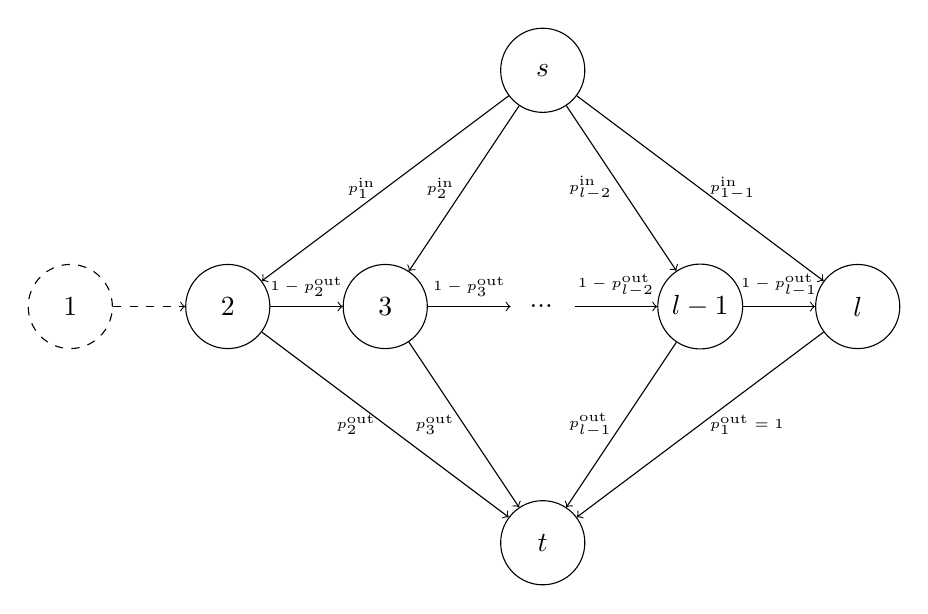
\begin{tikzpicture}
\node[dashdot] (1) at (0,0) {$1$};
\node[main] (2) at (2,0) {$2$};
\node[main] (3) at (4,0) {$3$};
\node[] (dots) at (6,0) { \vspace{2cm} ...  \vspace{2cm} };
\node[main] (lp) at (8,0) {${l-1}$};
\node[main] (l) at (10,0) {$l$};

\node[main] (s) at (6, 3) {$s$};
\node[main] (t) at (6, -3) {$t$};

\path [->] (s) edge node[left] {\tiny$p^\text{in}_{1}$} (2);
\path [->] (s) edge node[left] {\tiny$p^\text{in}_{2}$} (3);
\path [->] (s) edge node[left] {\tiny$p^\text{in}_{l-2}$} (lp);
\path [->] (s) edge node[right] {\tiny$p^\text{in}_{1-1}$} (l);

\path [->, dashed] (1) edge node[above] {} (2);
\path [->] (2) edge node[above] {\tiny$1 - p^\text{out}_{2}$} (3);
\path [->] (3) edge node[above] {\tiny$1 - p^\text{out}_{3}$} (dots);
\path [->] (dots) edge node[above] {\tiny$1 - p^\text{out}_{l-2}$} (lp);
\path [->] (lp) edge node[above] {\tiny$1 - p^\text{out}_{l-1}$} (l);

\path [->] (2) edge node[left] {\tiny$p^\text{out}_{2}$} (t);
\path [->] (3) edge node[left] {\tiny$p^\text{out}_{3}$} (t);
\path [->] (lp) edge node[left] {\tiny$p^\text{out}_{l-1}$} (t);
\path [->] (l) edge node[right] {\tiny$p^\text{out}_{1}=1$} (t);
\end{tikzpicture} 
\end{center}

qui est donc représentée par la matrice de transition $\mathbf{W}$ suivante :

\begin{equation}
\mathbf{W} = \left(
\begin{array}{c|ccccccc|c}
	0 & p^\text{in}_1 & p^\text{in}_2 & p^\text{in}_3 & \ldots & p^\text{in}_{l-3} & p^\text{in}_{l-2} & p^\text{in}_{l-1} & 0 \\
	\hline
	0 & 0 & 1 - p^\text{out}_{2} & 0 & \cdots & 0 & 0 & 0 & p^\text{out}_{2} \\	
	0 & 0 & 0 & 1 - p^\text{out}_{3} & \ddots & 0 & 0 & 0 & p^\text{out}_{3} \\
	0 & 0 & 0 & 0 & \ddots & 0 & 0 & 0 & p^\text{out}_{4} \\
	\rule{0pt}{18pt} \vdots & \vdots & \vdots & \vdots & \ddots & \ddots & \ddots & \vdots & \vdots \\
	\rule{0pt}{18pt} 0 & 0 & 0 & 0 & \cdots & 0 & 1 - p^\text{out}_{l-2} & 0 & p^\text{out}_{l-2} \\
	\rule{0pt}{15pt} 0 & 0 & 0 & 0 & \cdots & 0 & 0 & 1 - p^\text{out}_{l-1} & p^\text{out}_{l-1} \\
	\rule{0pt}{15pt} 0 & 0 & 0 & 0 & \cdots & 0 & 0 & 0 & p^\text{out}_{1} \\
	\hline
	\rule{0pt}{15pt} 0 & 0 & 0 & 0 & \cdots & 0 & 0 & 0 & 0
\end{array}
\right)
\end{equation}

Pour représenter le fait qu'une personne qui monte en $i$ va nécessairement en $i + 1$ avant de descendre, la probabilité de monter à l'arrêt $i$, i.e $p^\text{in}_i$, est directement connecté au noeud $i+1$. Le noeud représentant l'arrêt $1$ n'est donc plus nécessaire. \\

A partir de cette matrice, on peut calculer la \emph{matrice fondamentale}, $\mathbf{Z}$, de la façon suivante :

\begin{equation}
\mathbf{Z} := \mathbf{I} + \mathbf{W} + \mathbf{W}^2 + \mathbf{W}^3 + \ldots =  (\mathbf{I} - \mathbf{W})^{-1}
\end{equation}

Comme cette chaîne ne possède pas de boucle, on sait que les composantes de cette matrice $z_{kl}$ contiennent la \emph{probabilité d'atteindre $l$ en partant de $k$} (REF, p.ex. Saerens).  On a donc : 

\begin{equation}
z_{kl} = \begin{cases}
(1 - p^\text{out}_{k}) \cdots (1 - p^\text{out}_{l-1}) & \text{si } k < l \\
1 & \text{si } k = l \\
0 & \text{sinon}
\end{cases} \qquad \forall k, l \neq s, t
\end{equation}

la probabilité $f_{ij}$ s'obtient donc avec :

\begin{equation}
f_{ij} = p^\text{in}_i z_{i+1, j} p^\text{out}_j
\end{equation}

\subsection{Marges}

Les marges de $f_{ij}$ doivent vérifier $f_{i \bullet} = x_i / x_\bullet$ et $f_{\bullet j} = y_j / y_\bullet$. On a :

\begin{align}
f_{i \bullet} = \sum_{j=1}^l p^\text{in}_i z_{i+1, j} p^\text{out}_j = p^\text{in}_i \sum_{j=1}^l z_{i+1, j} p^\text{out}_j 
\end{align}
Comme $z_{i+1, j} p^\text{out}_j$ représente la probabilité d'avoir une trajectoire partant de $i+1$ et étant absorbé juste après avoir atteint $j$, on a :


\begin{align}
\sum_{j=1}^l z_{i+1, j} p^\text{out}_j &= 1 \\
\Rightarrow f_{i \bullet} = p^\text{in}_i &= \frac{x_i}{x_\bullet}
\end{align}

Pour l'autre marge, on fait par réccurence. Pour j = 2 :

\begin{align}
f_{\bullet 2} &= p^\text{in}_1 p^\text{out}_2 = \frac{x_1}{x_\bullet} \frac{y_2}{(x_1 - y_1)} \notag \\
			  &= \frac{x_1}{x_\bullet} \frac{y_2}{x_1} = \frac{y_2}{x_\bullet} = \frac{y_2}{y_\bullet}
\end{align}

En supposant que $f_{\bullet j} = y_j / y_\bullet$, calculons $f_{\bullet, j+1}$. Pour commencer, remarquons que :

\begin{align}
z_{kl} = \begin{cases}
z_{k, (l-1)} (1 - p^\text{out}_{l-1}) & \text{si } k < l \\
1 & \text{si } k = l \\
0 & \text{sinon}
\end{cases}
\end{align}

On a donc :

\begin{align}
f_{\bullet, (j+1)} &= \sum_{i=1}^l p^\text{in}_i z_{(i+1), (j+1)} p^\text{out}_{j+1} = \sum_{i=1}^{j-1} p^\text{in}_i z_{i+1, j} (1 - p^\text{out}_{j}) p^\text{out}_{j+1} + p^\text{in}_j p^\text{out}_{j+1} \notag \\
&= \frac{f_{\bullet, j}}{p^\text{out}_j}(1 - p^\text{out}_j)p^\text{out}_{j+1} + \frac{x_j}{x_\bullet} p^\text{out}_{j+1} = \left( \frac{y_j}{y_\bullet} \left( \frac{1}{p^\text{out}_j} - 1 \right)+ \frac{x_j}{x_\bullet} \right) p^\text{out}_{j+1} \notag \\
&= \left( \frac{n_{j-1,j} - y_j + x_j}{y_\bullet} \right) \frac{y_{j+1}}{n_{j,j+1}} = \frac{y_{j+1}}{y_\bullet}
\end{align}




\end{document}
